\section{Modello di Ising 1D}

Il modello di Ising 1D è uno dei pochi modelli della meccanica statistica che presenta una soluzione esatta.
Il reticolo che prendiamo in considerazione in questo caso è lineare, tale per cui ogni sito reticolare presenta 
solo due primi vicini. Lavorando con condizioni periodiche al contorno, l'N-esimo spin diventa un vicino del 
primo ed il sistema si chiude ad anello, come è possibile apprezzare in Figura \ref{fig: Ising1D_pbc}.

\begin{figure}[h!]
    \centering
    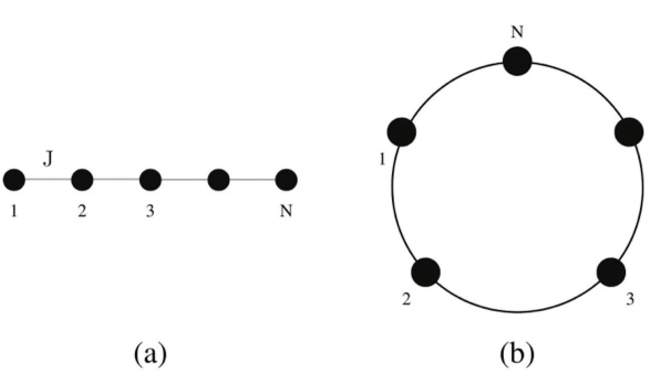
\includegraphics[width=0.7\textwidth]{Immagini/Ising1D_pbc.png}
    \caption{L'immagine (a) è un esempio di modello di Ising 1D senza pbc, mentre in (b) si può apprezzare 
    come la catena si chiuda su se stessa nel caso di condizioni periodiche al contorno. }
    \label{fig: Ising1D_pbc}
\end{figure}


\subsection{Soluzione esatta}

Considerare un sistema con condizioni periodiche al contorno, come (b) in Figura \ref{fig: Ising1D_pbc}, consente 
di scrivere l'Hamiltoniana in forma simmetrica come 

\begin{equation}
    H\,=\,-J\sum_{i} \sigma_i \sigma_{i+1}\,-\,\frac{h}{2}\sum_{i} \left(\sigma_i\,+\,\sigma_{i+1}\right),
    \label{eq: ising_ham_sim}
\end{equation}

dato che $\sigma_{N+1}\,=\,\sigma_1$. La funzione di partizione del sistema è data dalla somma su tutte le possibili 
configurazioni del sistema, che si traduce in 

\begin{equation}
    Q\left(h,\,T\right)\,=\,\sum_{\sigma_1=\pm 1} \cdots \sum_{\sigma_N=\pm 1} \exp{\left\{\beta\left[J\sum_i \sigma_i \sigma_{i+1}\,+\,\frac{h}{2}\sum_i \left(\sigma_i\,+\,\sigma_{i+1}\right)\right]\right\}}
    \label{eq: part_func}
\end{equation}

Definendo una matrice P come

\begin{equation}
    P = \begin{pmatrix}
    e^{\beta\left(J\,+\,h\right)} & e^{-\beta J} \\\\
    e^{-\beta J} & e^{\beta\left(J\,-\,h\right)}
    \end{pmatrix}
    \label{eq: mat_P}
\end{equation}

è possibile riscrivere la funzione di partizione in termini matriciali

\begin{equation}
    Q\left(h,\,T\right)\,=\,\sum_{\sigma_1=\pm 1} \cdots \sum_{\sigma_N=\pm 1} \langle \sigma_1 | P | \sigma_2 \rangle \langle \sigma_2 | P | \sigma_3 \rangle \cdots \langle \sigma_{N-1} | P | \sigma_N \rangle \langle \sigma_N | P | \sigma_1 \rangle 
    \label{eq: part_func_mat}
\end{equation}

Notando che sono presenti $N\,-\,1$ completezze, è possibile procedere ad una semplificazione estrema della relazione 
\eqref{eq: part_func_mat} che consente di apprezzare come la funzione di partizione altro non sia che la traccia della matrice P 
elevata alla N. 

\begin{equation}
    Q\left(h,\,T\right)\,=\,\sum_{\sigma_1=\pm 1} \langle \sigma_1 | P^N | \sigma_1 \rangle \,=\,Tr\left(P^N\right)\,=\,\lambda_1^N\,+\,\lambda_2^N,
    \label{eq: part_func_simp}
\end{equation}

dove $\lambda_1$ e $\lambda_2$ sono gli autovalori della matrice P. La loro determinazione richiede la soluzione di un problema agli 
autovalori, che porta a 

\begin{equation}
    \lambda_{1,2}\,=\,e^{\beta J} \cosh{\left(\beta h\right)}\,\pm\,\sqrt{e^{- 2 \beta J}\,+\,e^{2 \beta J} \sinh^2{\left(\beta h\right)}}.
    \label{eq: autoval_P}
\end{equation}

Una ottima approssimazione, quando il numero di spin preso in considerazione è elevato, consiste nel trascurare il secondo autovalore 
dato che 

\begin{equation}
    \lim_{N \to \infty} \left(\frac{\lambda_2}{\lambda_1}\right)^N\,=\,0.
    \label{eq: approx_Q}
\end{equation}

L'energia libera, dalla quale è possibile determinare tutta la termodinamica del sistema, risulta quindi

\begin{equation}
    A\left(h,\,T\right)\,=\,-k_B T \ln{\left[Q\left(h,\,T\right)\right]}\,\simeq\,-Nk_BT \ln{\left(\lambda_1\right)}.
    \label{eq: en_lib}
\end{equation}


\subsection{Teoria di Campo Medio}